%----------------------------------------------------------------------------
%----------------------------------------------------------------------------
We specify the position of the lasers on the dye laser table with respect to the output port and output surface (measured from the edge holes) of each laser. The YAG has three output ports; we will use the middle port for this experiment. The dye lasers have two ports - and input and output port. The output port is on the right if you are facing the front of the laser. The tolerance for these positions is $\pm\frac{1}{8}$ inch. See figure \ref{laser_positions}.
%----------------------------------------------------------------------------
% laser_positions.tex
% by Troy Hix, May 2005
%----------------------------------------------------------------------------
\begin{sidewaysfigure}
\center
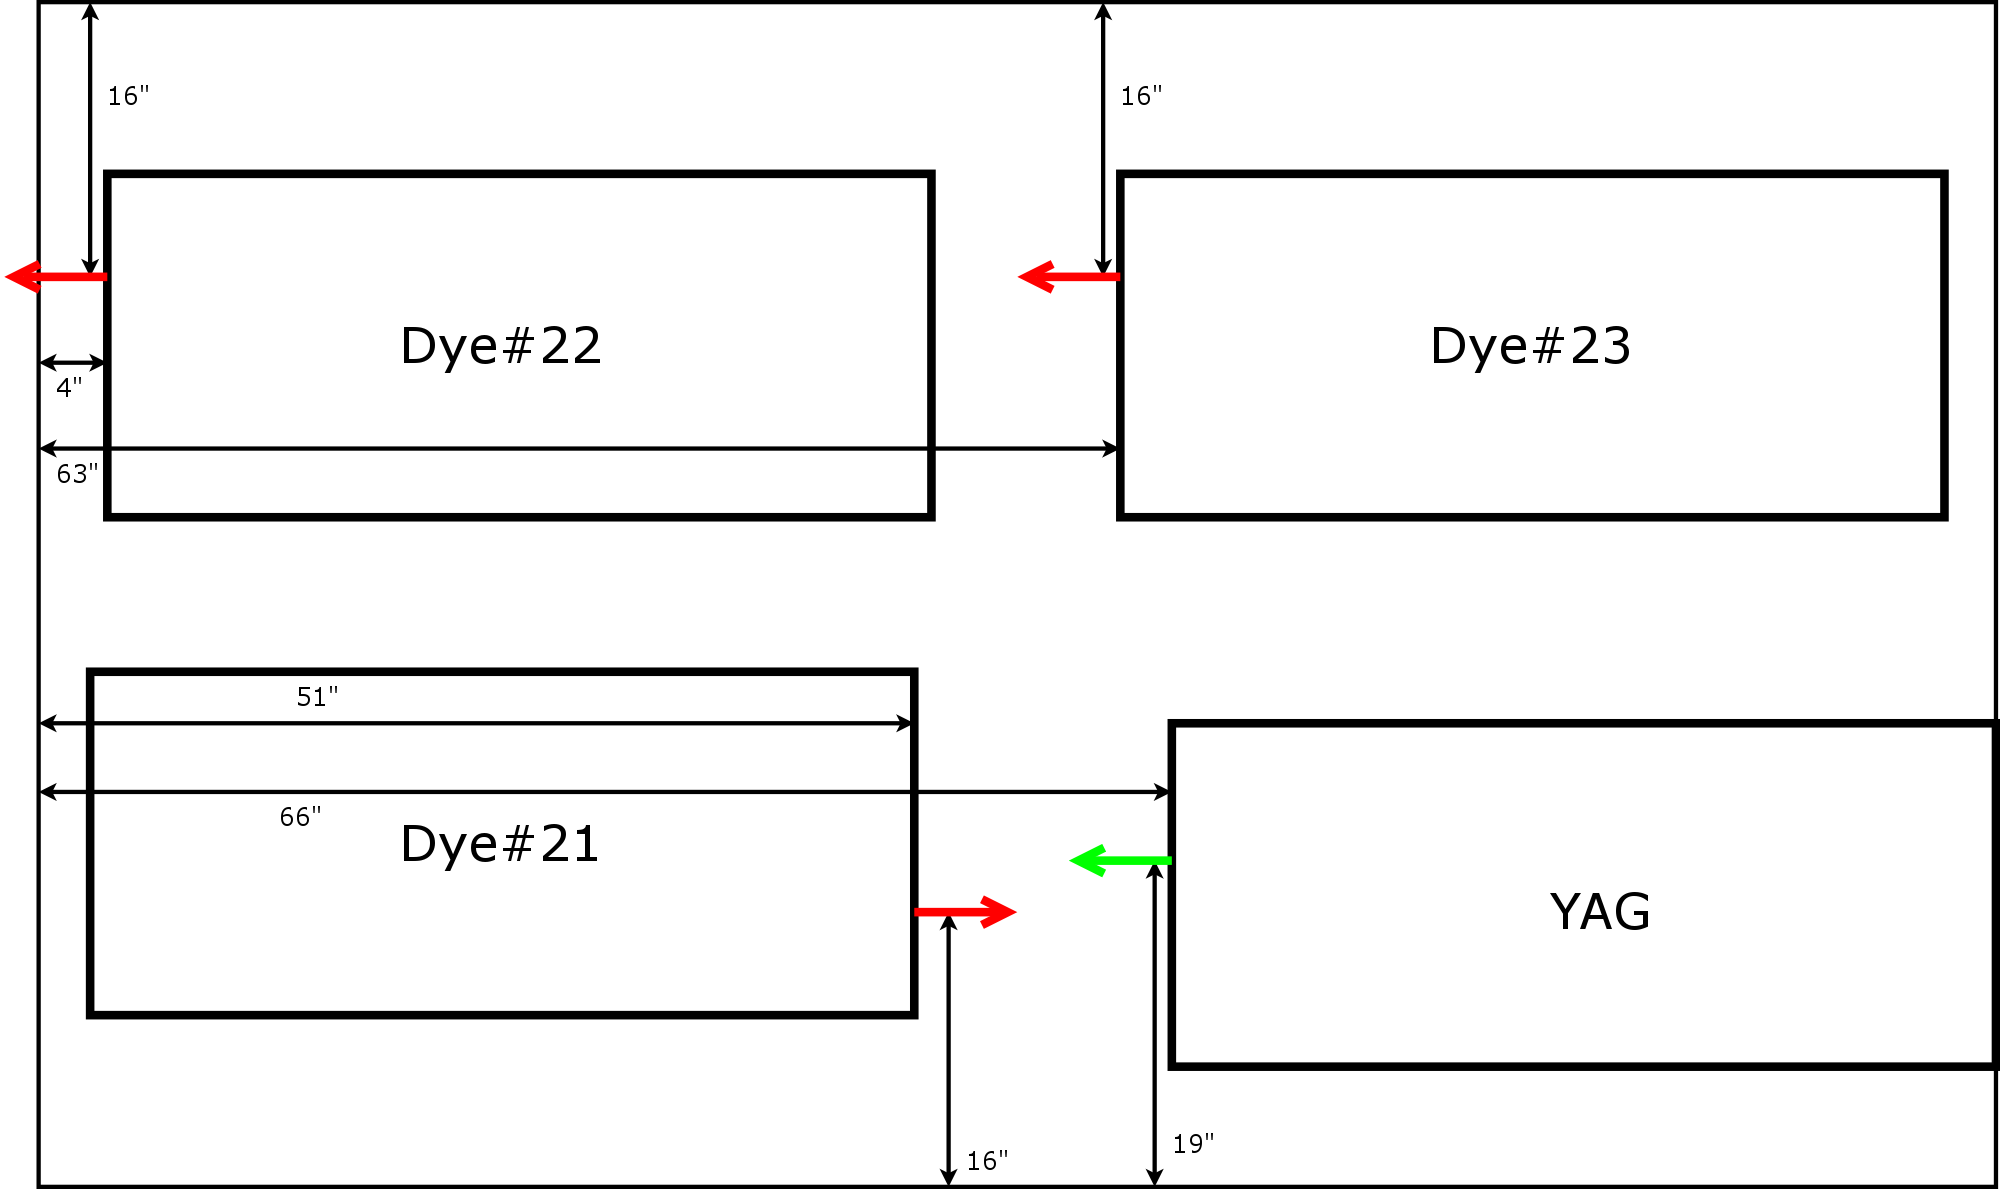
\includegraphics[width=7.75in]
{laser_positions/laser_positions.png}\\
\caption[Laser positions on dye laser table]{Laser positions on dye laser table. The outside border of the diagram (i.e., the reference edge for all dimensions) is the line defined by the last column (or row) of 1/4-20 tapped holes on the optical bench (NOT the actual edge of the table).}
\label{laser_positions}
\end{sidewaysfigure} 
%----------------------------------------------------------------------------
%----------------------------------------------------------------------------
%----------------------------------------------------------------------------



%----------------------------------------------------------------------------

The output from the Nd:YAG is split into three equal parts and sent to the input ports of each dye laser. First the beam is sent though a beam splitter that transmits two thirds of the incident beam power and reflects the remaining third. The transmitted beam is then sent though a beam splitter that transmits half and reflects half the incident beam power. In this way, we pump each dye laser with equal power allowing the most flexibility when exploring different pulse sequences. See figure \ref{YAG_positions}
%----------------------------------------------------------------------------
% YAG_positions.tex
% by Troy Hix, May 2005
%----------------------------------------------------------------------------
\begin{sidewaysfigure}
\center
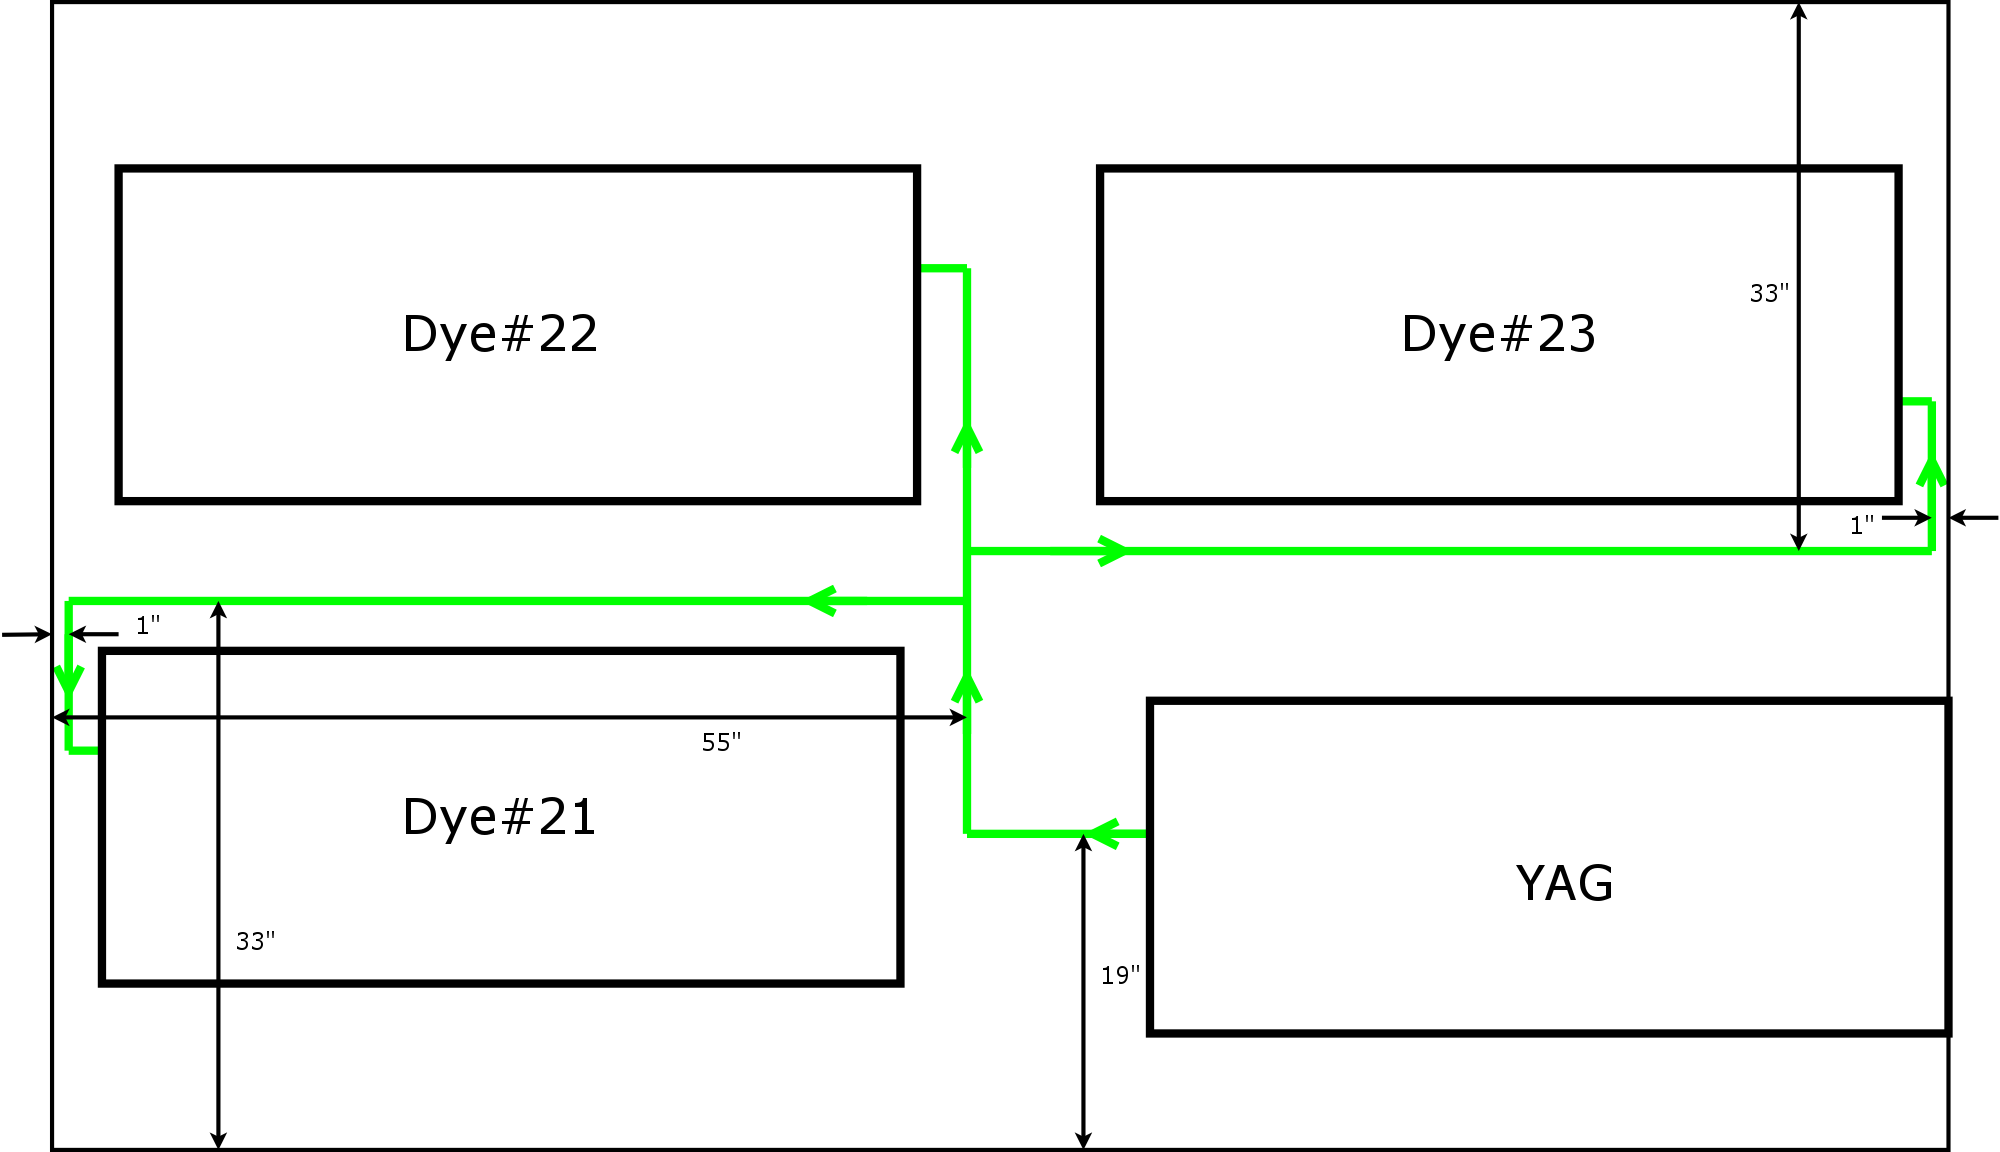
\includegraphics[width=7.75in]
{YAG_positions/YAG_positions.png}\\
\caption{YAG beam positions}
\label{YAG_positions}
\end{sidewaysfigure} 
%----------------------------------------------------------------------------
%----------------------------------------------------------------------------
%----------------------------------------------------------------------------



%----------------------------------------------------------------------------

The output from each dye laser is conditioned with respect to polarization and amplitude before it leaves the dye laser table. This is mainly for safety reasons, but also has the added advantage of localizing the Pockels cell system, along with its associated fast high voltage electronics, far from the data acquisition region of the experiment. The relative delay between each beam is adjusted on the dye laser table to allow for a convenient beam line on the next two tables. See figure \ref{dye_positions}.
%----------------------------------------------------------------------------
% dye_positions.tex
% by Troy Hix, May 2005
%----------------------------------------------------------------------------
\begin{sidewaysfigure}
\center
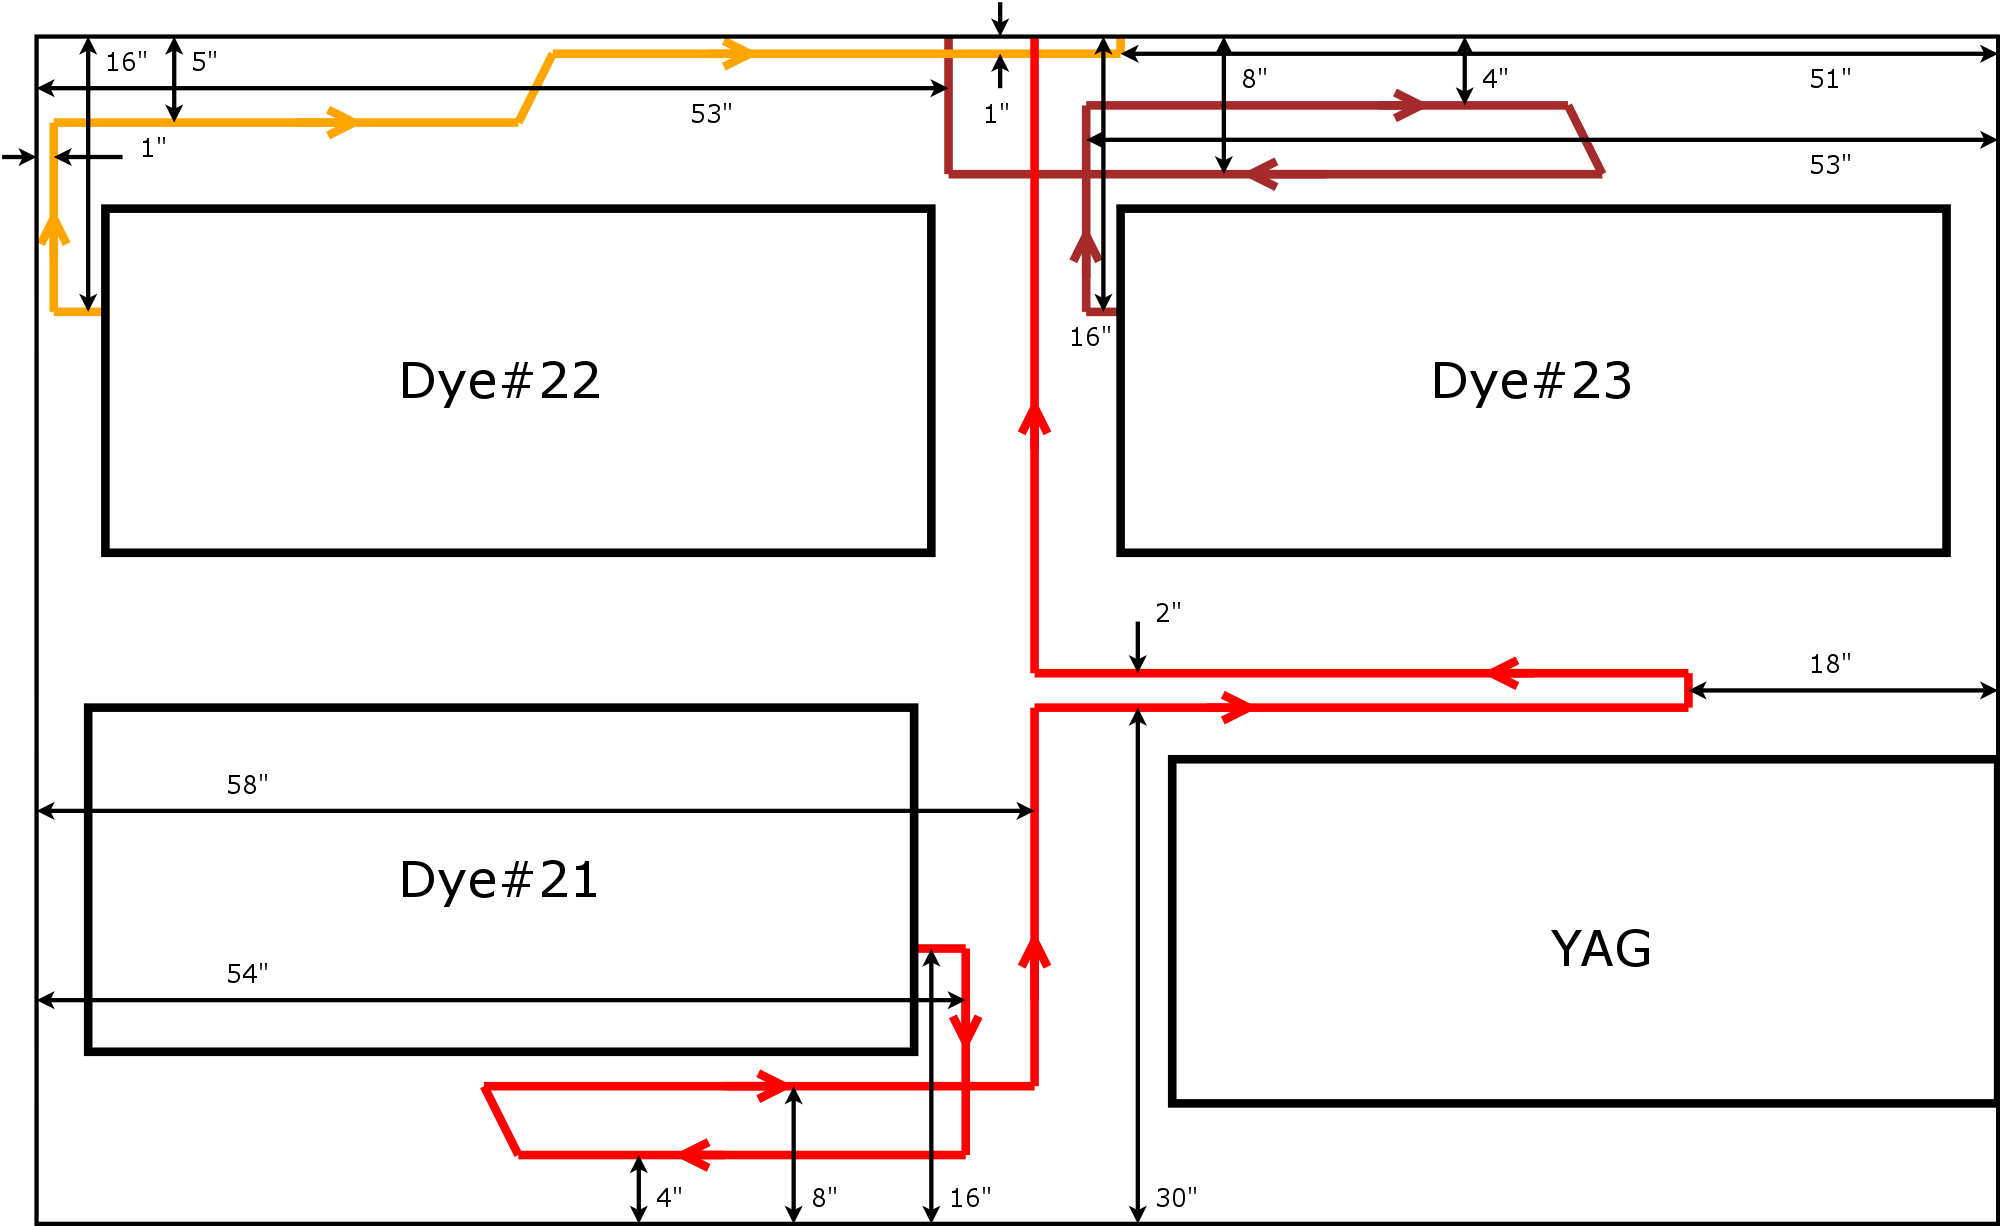
\includegraphics[width=7.75in]
{dye_positions/dye_positions.png}\\
\caption{Dye beam positions}
\label{dye_positions}
\end{sidewaysfigure} 
%----------------------------------------------------------------------------
%----------------------------------------------------------------------------
%----------------------------------------------------------------------------



%----------------------------------------------------------------------------

The Pockels cell system consists of a pile-of-plates polarizer, a Pockels cell, then a Brewster plate. The output of the pile-of-plates will be highly polarized in the horizontal direction. When switched, the Pockels cell will rotate this horizontal polarization toward the vertical by a specified amount. The Brewster plate will then output a sample of the vertical component of this beam. In this way we produce a vertically polarized output beam with continuously selectable pulse energy. See figure \ref{dye_mileposts}
%----------------------------------------------------------------------------
% dye_table_mileposts.tex
% by Troy Hix, May 2005
%----------------------------------------------------------------------------
\begin{sidewaysfigure}
\center
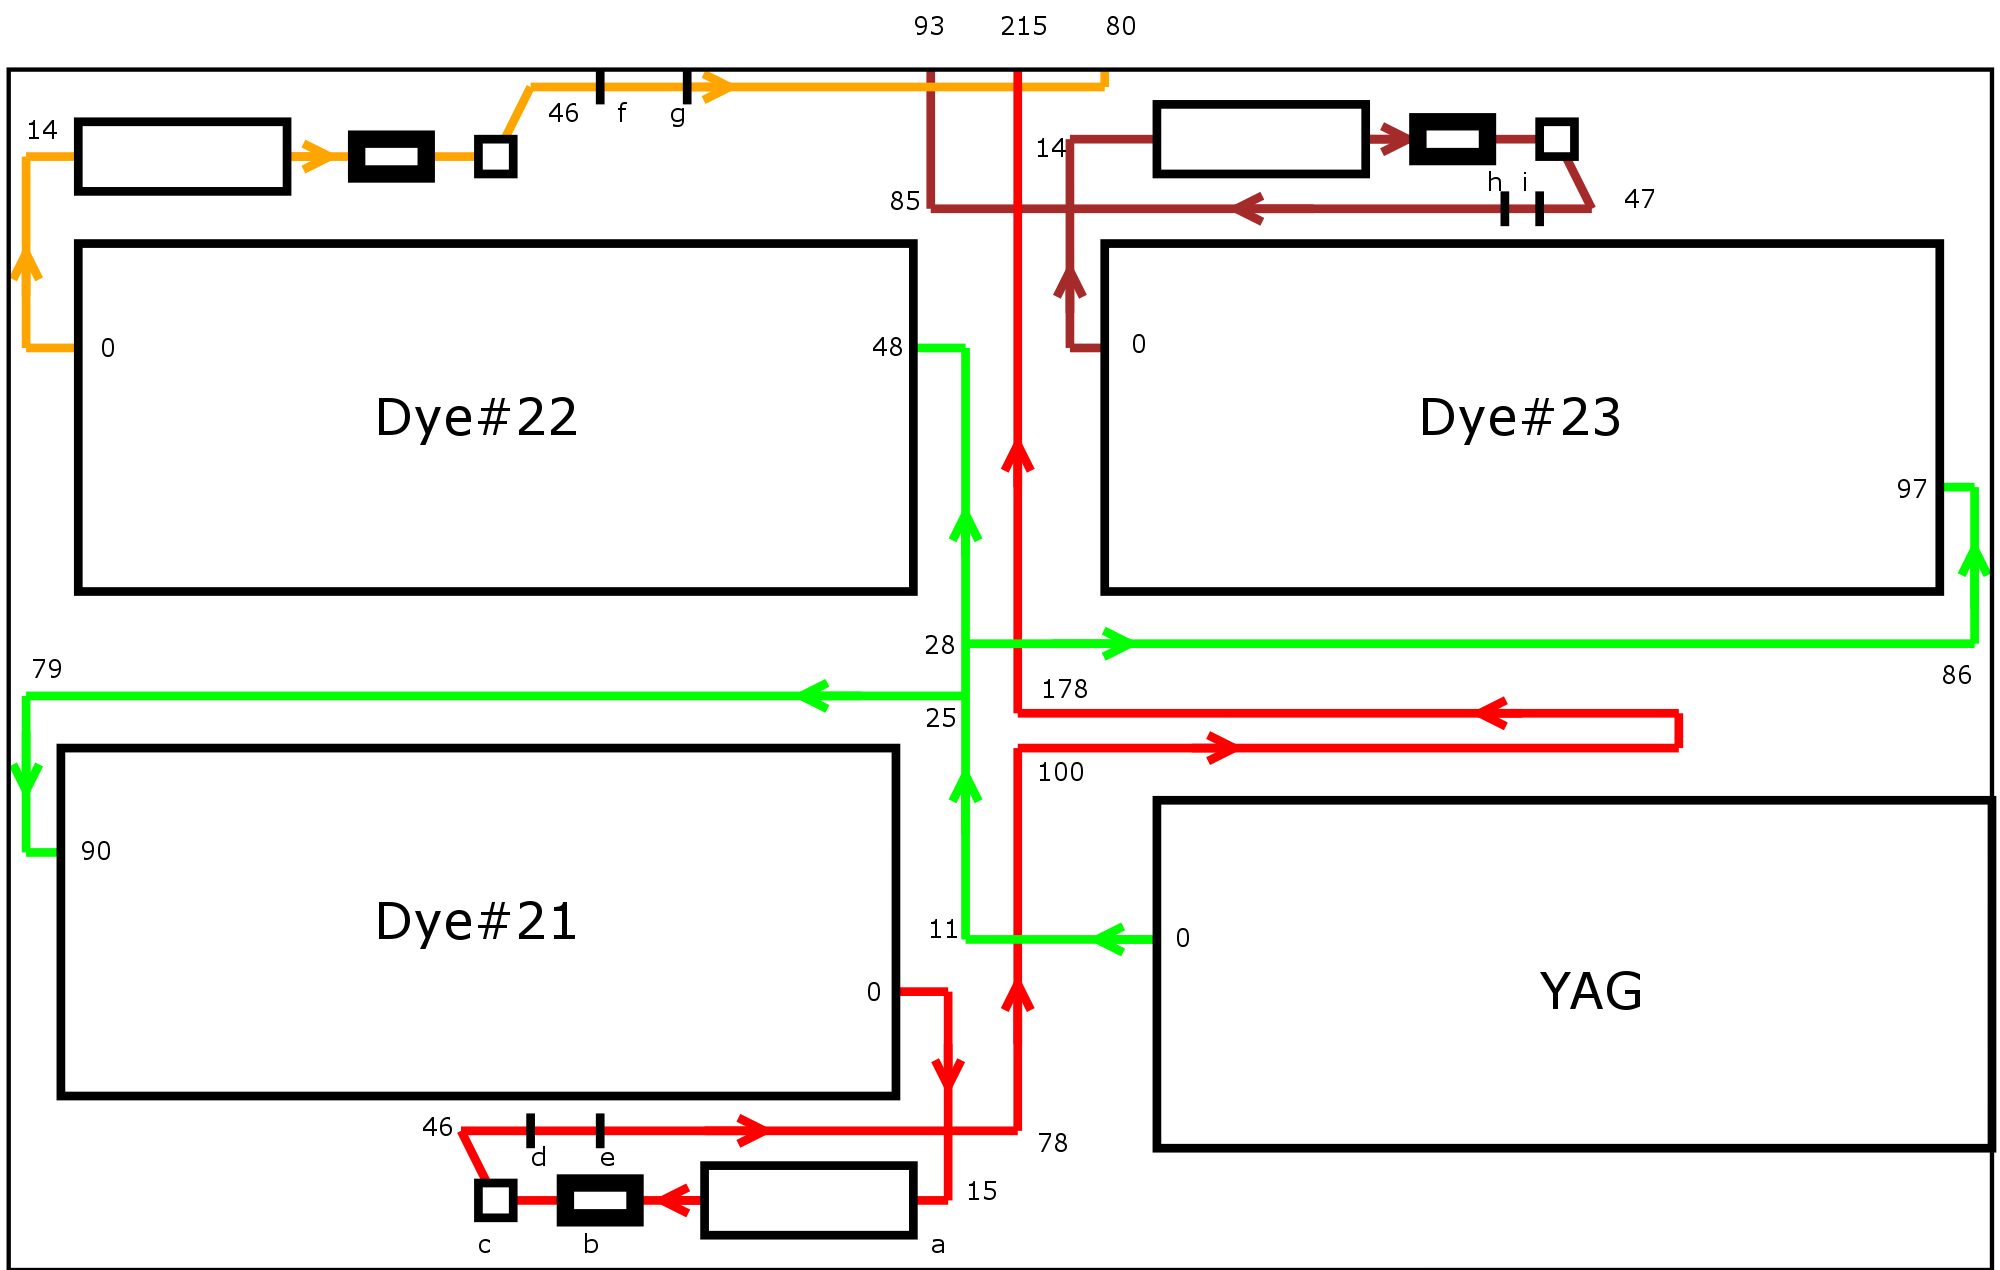
\includegraphics[width=7.75in]
{dye_mileposts/dye_mileposts.png}
\caption[Beam mileposts and optics on the dye laser table]{Beam mileposts and optics on the dye laser table. the mileposts along each beam line is given in inches. Optic (a) is a pile-of-plates polarizer; (b) Pockels cell, (c) Brewster plate, (d) +1 m lens at mile post 50, (e) -1 m lens at milepost 54, (f) +1 m lens at milepost 50, (g) -1 m lens at milepost 55, (h) +1 m lens at milepost 50, (i) -1 m lens at milepost 52.5.}
\label{dye_mileposts}
\end{sidewaysfigure} 
%----------------------------------------------------------------------------
%----------------------------------------------------------------------------
%----------------------------------------------------------------------------



%----------------------------------------------------------------------------
%----------------------------------------------------------------------------
%----------------------------------------------------------------------------
%----------------------------------------------------------------------------
%----------------------------------------------------------------------------
